\section{Preprocessing}

When capturing an image using a dermatoscope the skin is illuminated equally over the skin area to be photographed. The dermatoscope captures hi-resolution images with low levels of noise. The amount of preprocessing required is limited to colour enhancement to achieve better segmentation results. Using a digital camera like those found in smartphones requires introduces other challenges \cite{auto_seg}.

Unequal illumination or shadows in the image can make it more difficult for the segmentation algorithm to precisely recognise the lesions border. Glare from too much illumination, noise introduced by the circuitry of the sensor in the digital camera or hairs on the skin can also make it difficult to differentiate between the lesion area and healthy skin.

The preprocessing stage attempts to reduce the interference cause by these factors.


\subsection{Equalization}

\begin{figure}[H]
    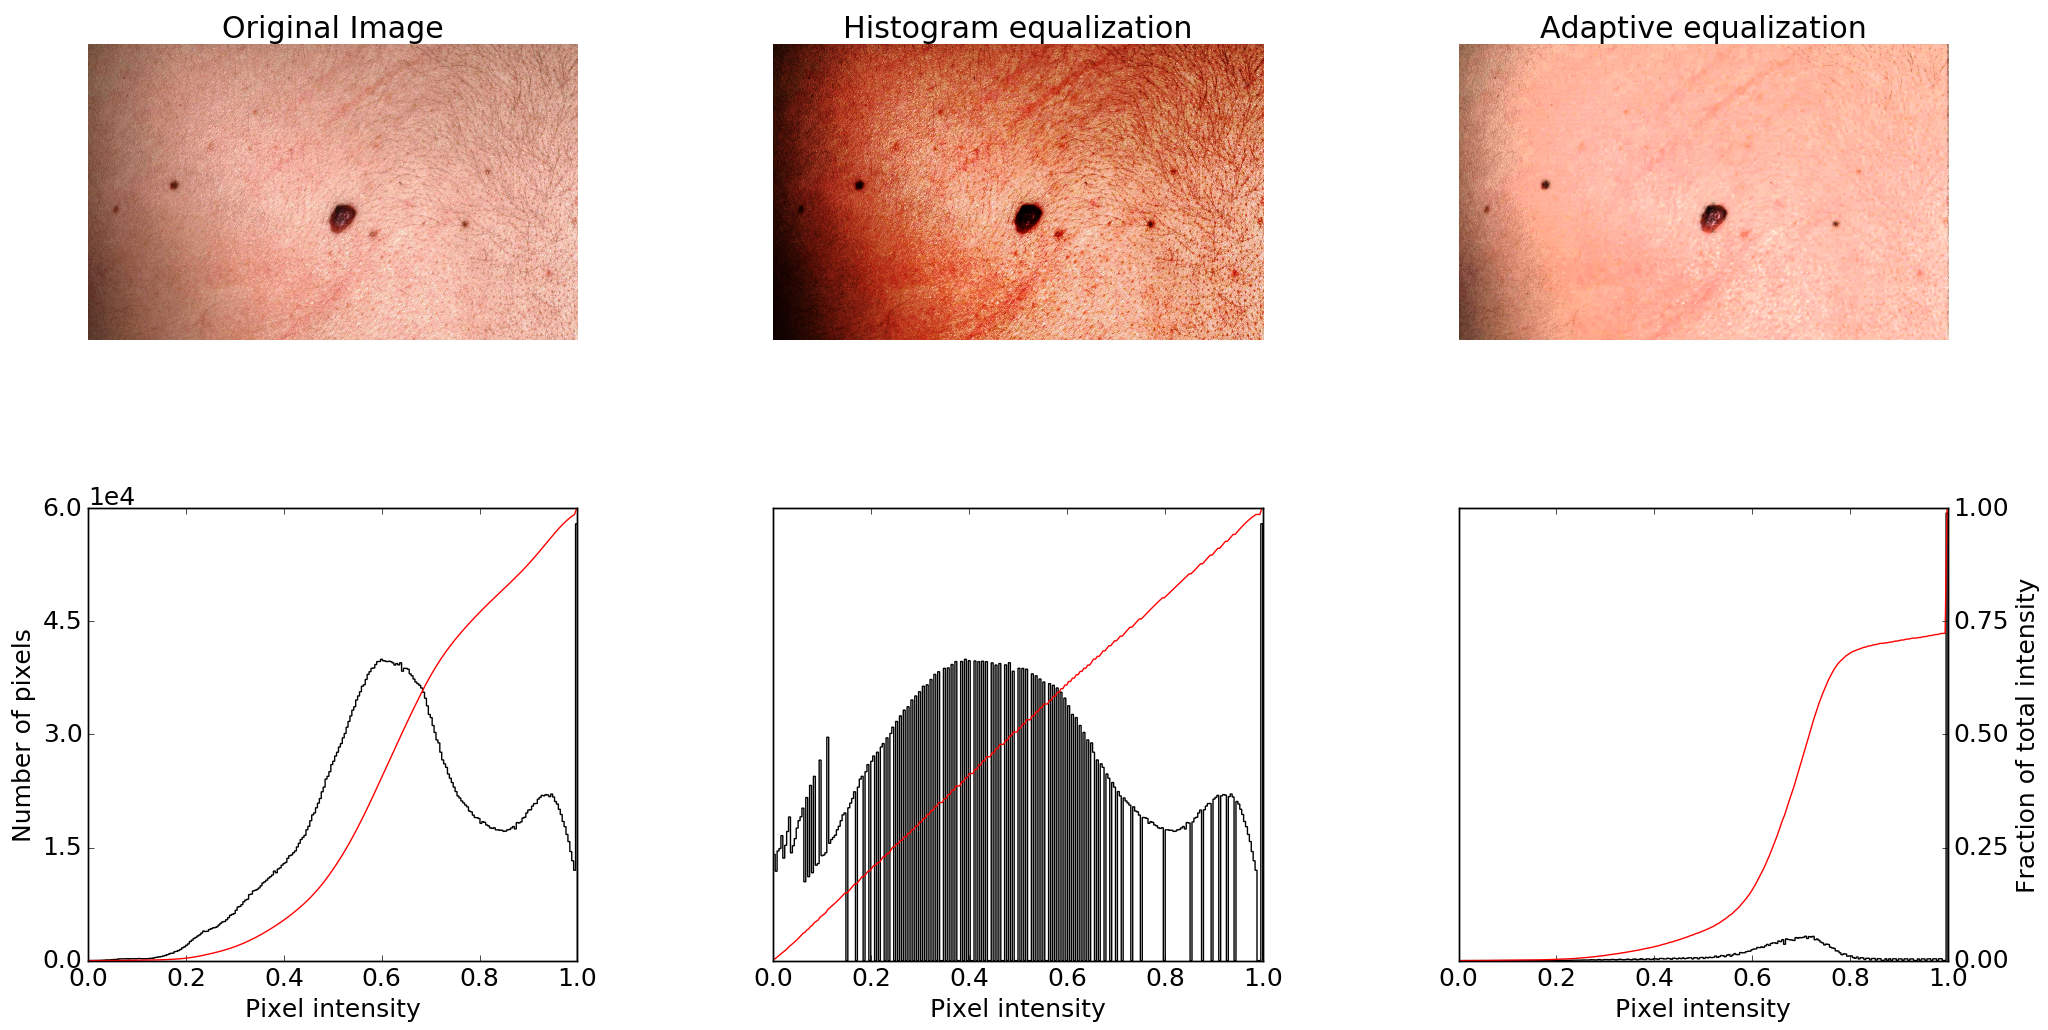
\includegraphics[width=\textwidth,keepaspectratio]{assets/image_processing/equalization/figure_01.png}
    \caption{Image Equalization Example A}
    \label{fig:eq_A}
\end{figure}
\begin{figure}[H]
    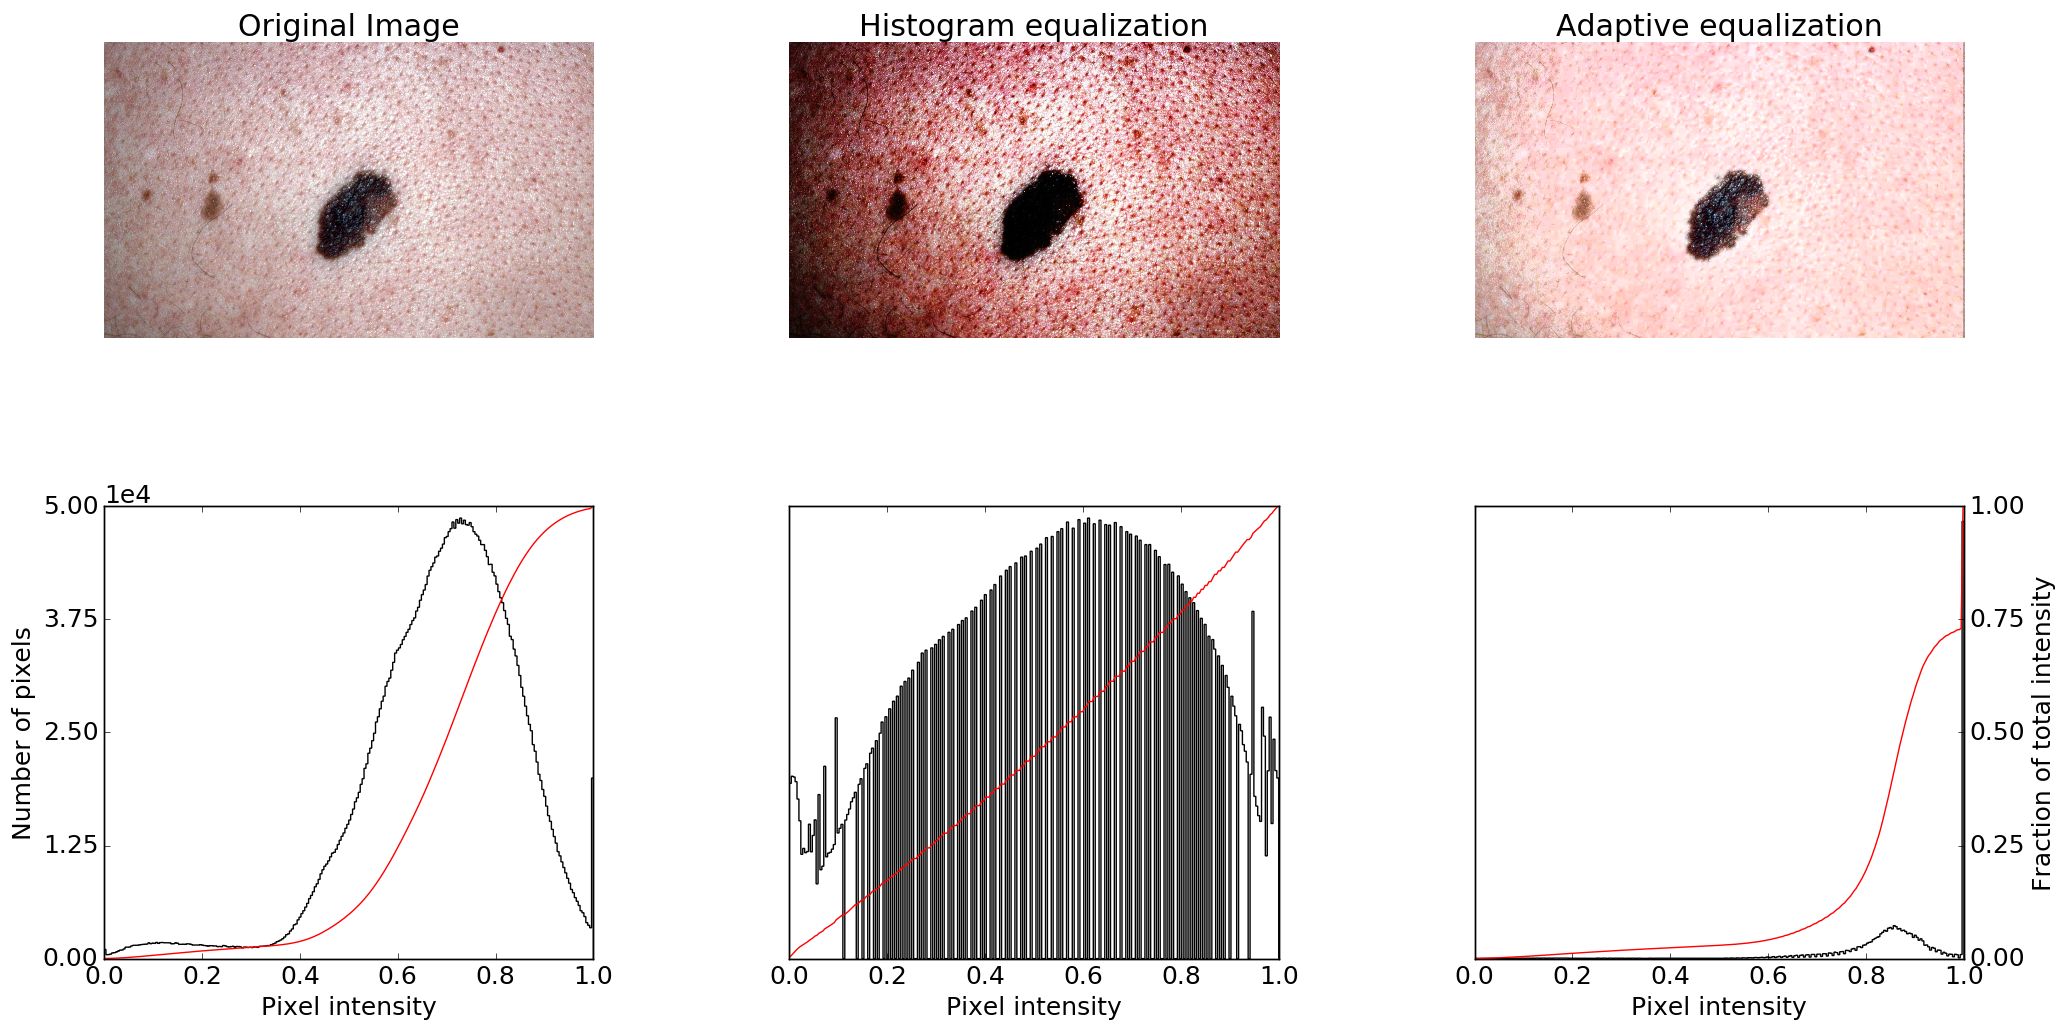
\includegraphics[width=\textwidth,keepaspectratio]{assets/image_processing/equalization/figure_02.png}
    \caption{Image Equalization Example B}
    \label{fig:eq_A}
\end{figure}
\begin{figure}[H]
    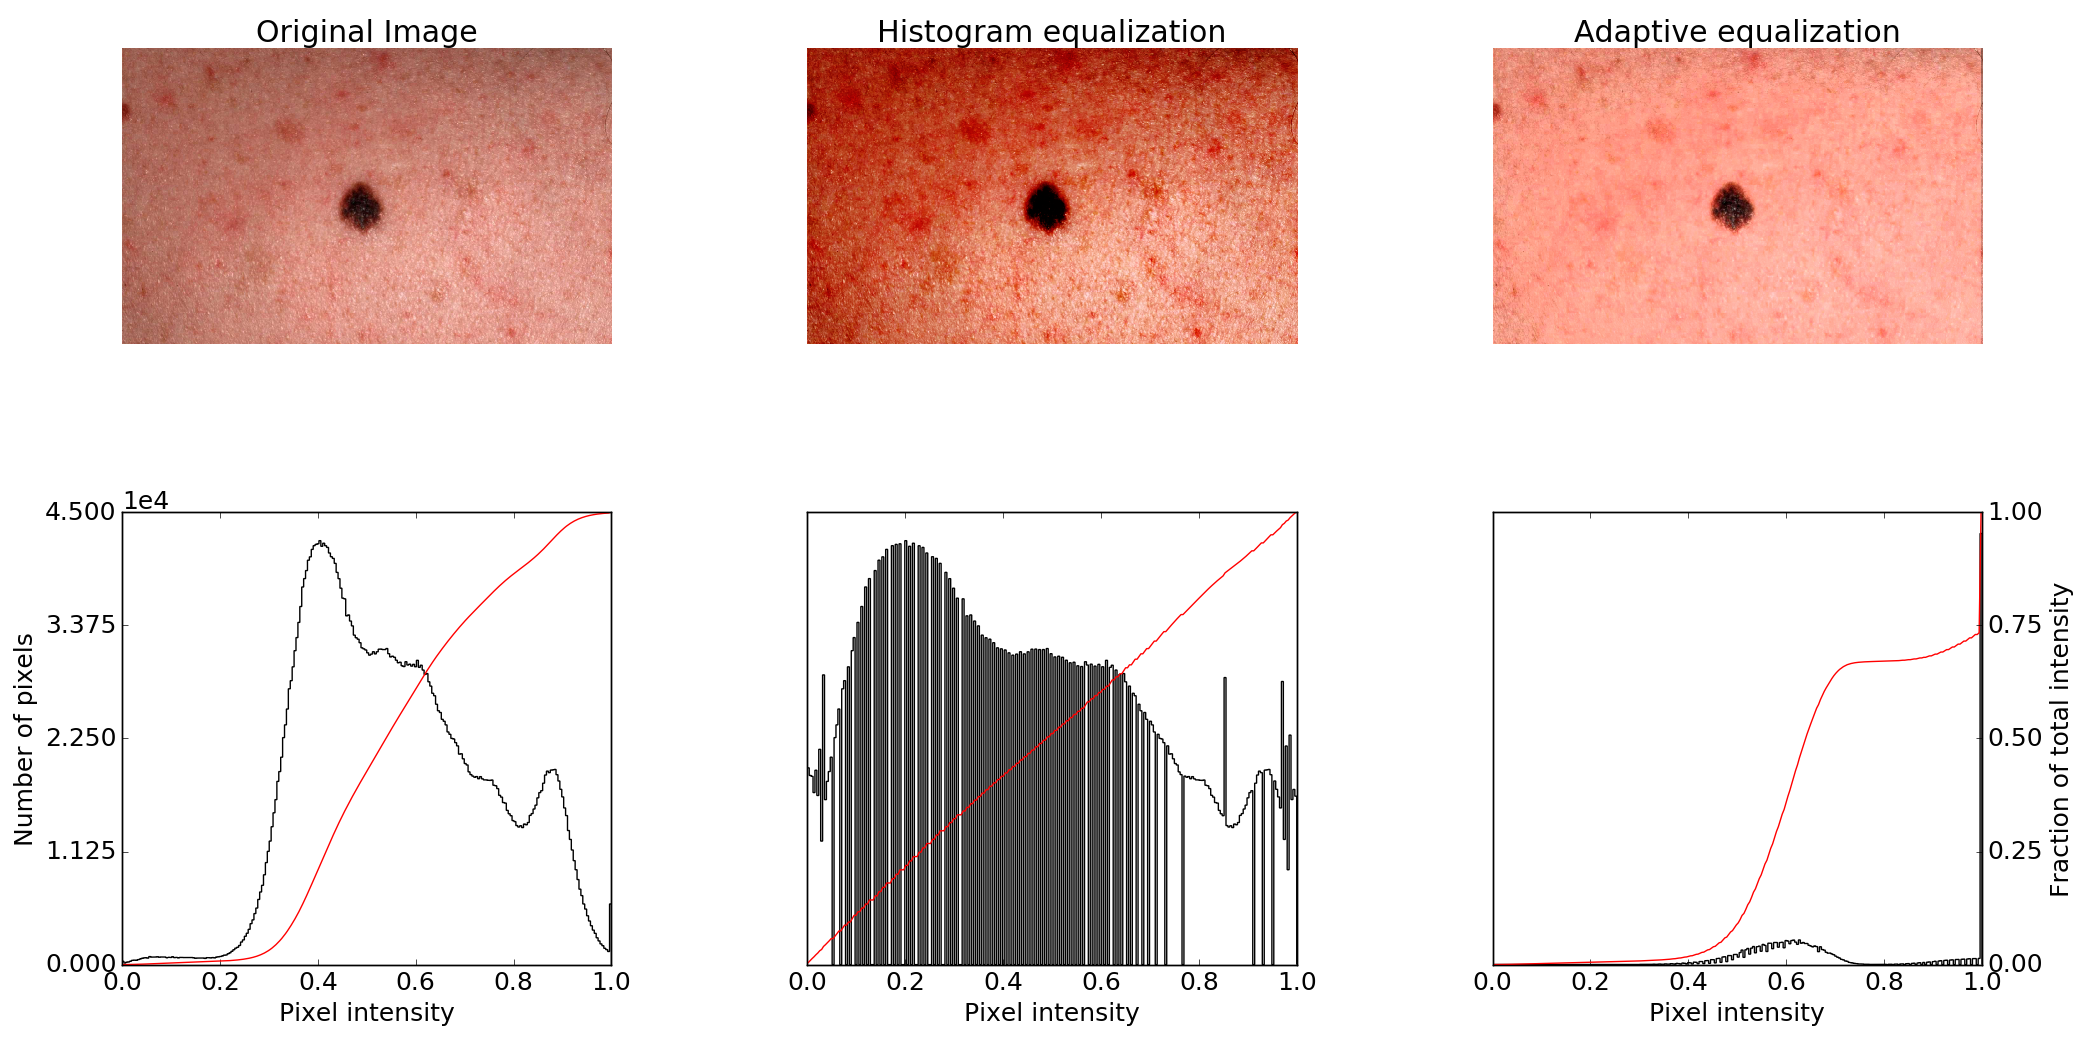
\includegraphics[width=\textwidth,keepaspectratio]{assets/image_processing/equalization/figure_03.png}
    \caption{Image Equalization Example C}
    \label{fig:eq_A}
\end{figure}

\subsection{Median Blur}
\subsection{Gaussian Blur}